\chapter[Proposed Methods]{Proposed Methods: Weighted sampling schemes towards diversified generation in Gen-RKM}
\label{chap-methods}
\chaptermark{Proposed Methods}
As discussed in the literature review section, the unbalanced data problem could occur in either supervised or unsupervised scenarios. In this chapter, We propose methods to address the problem within the framework of Gen-RKM under both the two settings.


\section{Mitigating data imbalance in supervised setting}
\label{sec-methods-supervised}
Normally, classic strategies like class re-sampling or re-weighting (cost-sensitive training) can both be applied to address data imbalance issues in supervised learning settings. However, in the context of the unique architecture of Gen-RKM, where the final latent space is derived by performing SVD on the entire training dataset following the acquisition of the feature map and pre-image map, the re-weighting approach is ineffective. This is because re-weighting on the RKM loss function only affects the weights of the feature map and pre-image map via backpropagation, and does not impact the final SVD process. Consequently, re-sampling methods are primarily investigated in this context.

\subsection{Inverse frequency sampling}
Consider a training dataset $\bD_{\text{train}} = \{ (\bx_i, \by_i) \}_{i=1}^N$, where $(\bx, \by)$ is the pair of feature and target, $\bx_i$ the feature vector of the $i$th sample, $\by_i \in (0, 1)^c$ the corresponding one-hot target vector over $c$ classes, and $N$ the number of samples in the training set. The sampling weights can be obtained simply by calculating the reciprocal of the frequency of the target classes: $w_i = 1/\text{count}(\by_i)$. The sampling probability is, therefore, $p_i=w_i/\sum_{i=1}^N w_i$. Instead of uniformly sampling data from the training set during the training phase, data points from the minor classes would be sampled with a higher probability than those from the major classes. Therefore, the distribution of training data is modified to achieve a more balanced representation across all classes.

\subsection{Inverse frequency sampling in the framework of Gen-RKM}
The detailed sampling procedure based on inverse frequency sampling in Gen-RKM is illustrated in this subsection. Although inverse frequency sampling is the most classic and straightforward method, adjustments are necessary when applying it to Gen-RKM due to the model’s unique architecture. Since the final step of RKM training requires an SVD on the full training set to obtain the latent space, re-sampling is not only needed at the beginning of every mini-batch but also before the last SVD step on the full training set. The detailed training step is shown below in algorithm \ref{alg-invs-rkm}.
\begin{algorithm}[H]
\caption{inverse frequency sampling for one-view Gen-RKM (Dual)}
\label{alg-invs-rkm}
\begin{algorithmic}[1]
\Require training data $\bD = \{\bx_i, \by_i\}_{i=1}^{N}$; mini-batch size $m$; \\
regularization parameters $\eta, c_{\text{stab}}, \gamma$; \\
explicit feature map $\bphi_{\boldsymbol{\theta}}(.)$ and explicit pre-image map $\bpsi_{\boldsymbol{\zeta}}(.)$; \\
dimension of latent space $s$;
\LComment{Compute Inverse weight}
\State $w_i \gets \frac{1}{count(\by_i)}$ \Comment{the reciprocal of the frequency of $\by_i$}
\State $p_i \gets w_i / \sum_{i=1}^n w_i$
\LComment{Training loop}
    \For{each epoch}
        \For{each mini-batch}
        \State $B \gets$ sample a mini-batch of size $m$ with probability $\boldsymbol{x}_i \sim p_i$ 
        \State do step 6-11 in algorithm \ref{alg-gen-rkm-dual}
        \EndFor
    \EndFor
\LComment{Final step to get all latent variables on modified full dataset}
\State $\bD_{\text{resampled}} \gets$ resample a size $N$ dataset from $\bD$ with probability $\bx_i \sim p_i$ 
\State repeat step 7-9 in algorithm \ref{alg-gen-rkm-dual}  on $\bD_{\text{resampled}}$
\end{algorithmic}
\end{algorithm}


\subsection{Extension to conditional generation in Gen-RKM}
\label{subsec-methods-congen}
Conditional generation involves generating new data samples based on certain attributes. A ubiquitous technique in combating data imbalance is the use of conditional generation with deep generative model. By learning the underlying data distribution via deep architecture, one can augment minority modes (or classes) with highly realistic synthetic data. Both VAE and GAN have their own modified version for conditional modeling, known as CVAE\cite{sohnLearningStructuredOutput2015} and CGAN\cite{mirzaConditionalGenerativeAdversarial2014}, respectively. However, the implementation of conditional generation within the framework of Gen-RKM has not yet been explored. Here, We propose a simple yet effective modified generation procedure aimed at achieving structured output representation in Gen-RKM ,as outlined in algorithm \ref{alg-con-gen-rkm}.

Let $\bH$ as a collection of latent variables and $\bY$ as the corresponding class labels for each data point. Recall that generation is based on random sampling from a trained GMM on latent variables in vanilla Gen-RKM:
\begin{equation}
    \bh^{*}\sim p(\bh) = \sum_{k=1}^{l}\pi_k\Normal(\bh | \bmu_{\bh,k},\bSigma_{\bh,k}).
\end{equation}
Instead of fitting GMM merely on $\bH$, we consider modeling the joint PDF of $\bh$ and $\by$ on a concatenated matrix : $\bH_{cat} = [\bH^\top; \bY^\top]^\top$. To obtain the generation conditioned on a certain class label, it is natural to sample from the conditional distribution $p(\bh|\by)$. One can verify that the conditional distribution of a mixture of Gaussian results in another GMM :
\begin{equation}
    p(\bh | \by) = \sum_{k=1}^{l}\pi_k^{\prime}\Normal(\bh | \bmu_{\bh|\by,k},\bSigma_{\bh|\by,k}).
\end{equation}
with the updated weights for each Gaussian component,
\begin{equation}
    \pi_k^{\prime} = \frac{\pi_k \Normal(\by|\bmu_{\by,k},\bSigma_{\by\by,k})}{\sum_{v=1}^{l}\pi_{v}\Normal(\by | \bmu_{\by,v},\bSigma_{\by\by,v})}.
\end{equation}
The more detailed derivation is shown in appendix \ref{A-conGMM}.
% Recall that the vanilla generation procedure in Gen-RKM is based on random sampling from a trained GMM on latent variables. 
\begin{algorithm}[H]
\caption{Conditional generation algorithm in Gen-RKM}
\label{alg-con-gen-rkm}
\begin{algorithmic}[1]
    \Require trained explicit pre-image map $\bpsi_{\boldsymbol{\zeta}}(.)$, interconnection matrix $\bW$; \\
    latent variables $\bH = [\bh_1,\dots,\bh_N] \in \bbR^{d\times N}$; \\
            class labels for each data point $\bY = [\by_1,\dots,\by_N] \in \bbR^{c\times N}$ (in one-hot encoding form, $c$ is the number of classes);\\
            conditioned class label $\by \in \bbR^{c}$ (in one-hot encoding form);\\
            number of Gaussian components in GMM $l$;
    \State $\bH_{cat} \gets [\bH^\top; \bY^\top]^\top \in \bbR^{(d+c)\times N}$
    \State $p(\bh,\by) \gets \text{GMM}_{l}(\bH_{cat})$
    \State $\bh^* \sim p(\bh|\by)$
    \State $\bx_{\text{gen}} \gets \bpsi_{\boldsymbol{\zeta}}(\bW \bh^{*})$
\end{algorithmic}
\end{algorithm}

This modification is inspired by the observation that, in the latent space, the latent variables of different class labels tend to cluster together, as shown in Figure \ref{fig-latent-ub}. Therefore, if we can sample from a selected sub-cluster, we are able to generate data conditioned on a particular label. Notice that this algorithm will fail if latent variables with different labels are intermixed in the latent space. It is advised to include label information as the second view in the training phase before conditional generation because latent representation would become more separated based on their categories, as pointed out in \cite{pandeyGenerativeRestrictedKernel2021}.


\section{Mitigating data imbalance in unsupervised setting}
\label{sec-methods-unsupervised}
Generative learning is typically conducted under an unsupervised manner, which means no label information is involved during the learning process. However, data imbalance problem might still exist even though it is hard to be clearly identified. More specifically, regions of the data space with fewer data points might be overlooked in the generative model, resulting in biased or unfair generation.  Inspired by the successful implementation of ridge leverage scores (RLS) sampling in combating mode collapse problem in GAN \cite{schreursLeverageScoreSampling2022}, we propose to incorporate the RLS sampling as a diversity sampling technique within the framework of Gen-RKM when label information is not available. The basic theoretical aspects of RLS and the modified training algorithm based on RLS sampling will be discussed below

\subsection{Ridge leverage score sampling}
Given a data matrix $\bX = [\bx_1,\dots,\bx_N]$ with size $d\times N$, the classical leverage score for the $i$th data point is defined as the $i$th diagonal element value of the projection matrix of $\bX$:
\begin{equation}
    l_{i} = \bx_i^\top (\bX\bX^\top)^{-1}\bx_i.
\end{equation}
Leverage score measures the importance or the influence of an individual observation within the dataset. Historically, it has been widely used for model diagnostics and assessment in classical regression models. Ridge regression is a penalized version of linear regression by including an additional L2 regularization term into the loss objective, its corresponding ridge leverage score for the $i$th observation is given by  
\begin{equation}
    l_{i}^{R}(\gamma) = \bx_i^\top (\bX\bX^\top + \gamma\mathbf{I})^{-1}\bx_i
\end{equation}
where $\gamma > 0$ is known as the regularization parameter in ridge regression. The additional regularization term $\gamma\mathbf{I}$ serves as stabilizing the ill-posed inversion problem in the above expression. Ridge regression can be readily integrated with kernel methods, which is essentially a simplified version of support vector regression \cite{vovkKernelRidgeRegression2013}. Given a feature map $\bvarphi(.)$ with its corresponding similarity metric $K(x,y)=\bvarphi(x)^\top\bvarphi(y)$, the leverage scores of kernel ridge regression can be expressed in a primal-dual form:
\begin{equation}
l_{i}^{KR}(\gamma) = 
    \begin{cases} \text{Primal:} \quad
\bvarphi(\bx_i)^\top(\bS_{\bvarphi}+\gamma\mathbf{I})^{-1}\bvarphi(\bx_i) 
\\
\text{Dual:} \quad
(\bK_{\bvarphi}(\bK_{\bvarphi}+\gamma\mathbf{I})^{-1})_{ii}
    \end{cases}
\end{equation}
Where $\mathbf{K}$ is the gram matrix with respect to similarity metric $K(.,.)$ and $\mathbf{S}_{\bvarphi} = \sum_{i=1}^{N}\bvarphi(\bx_i)\bvarphi(\bx_i)^\top$ is proportional to the sample covariance matrix. Depending on different data sizes and feature map dimensions, one can choose to leverage either primal or dual form to ensure optimal computational efficiency. 

In addition to a regression model diagnostic tool, RLS is crucial for sampling diverse landmarks in low-rank approximation problems, e.g., Nystr\"{o}m approximation for kernel matrices \cite{fanuelDiversitySamplingImplicit2021, mccurdyRidgeRegressionProvable2018}.  Schreurs et al. also illustrate the effectiveness of implementing RLS sampling in mitigating generation biases brought by unbalanced training data in the framework of GAN \cite{schreursLeverageScoreSampling2022}. Once the leverage scores are computed, one can immediately deduce the sampling probability for each data point via normalization on the leverage scores: $p_i = l^{KR}_i / \sum_{j=1}^N l^{KR}_j$. Ideally, minority modes tend to have higher leverage scores, making these points more likely to be oversampled, resulting in a more uniform-like distribution of the resampled data. A motivating example is presented in figure \ref{rls-demo}. One can observe that samples from minority modes generally share higher RLSs and the RLSs for the majority group are very close to zero, thus RLS sampling could automatically oversample minority modes while data points from the majority group are downsampled. In this spirit, problem of imbalance could be resolved by RLS sampling.

\begin{figure}[ht]
    \centering
    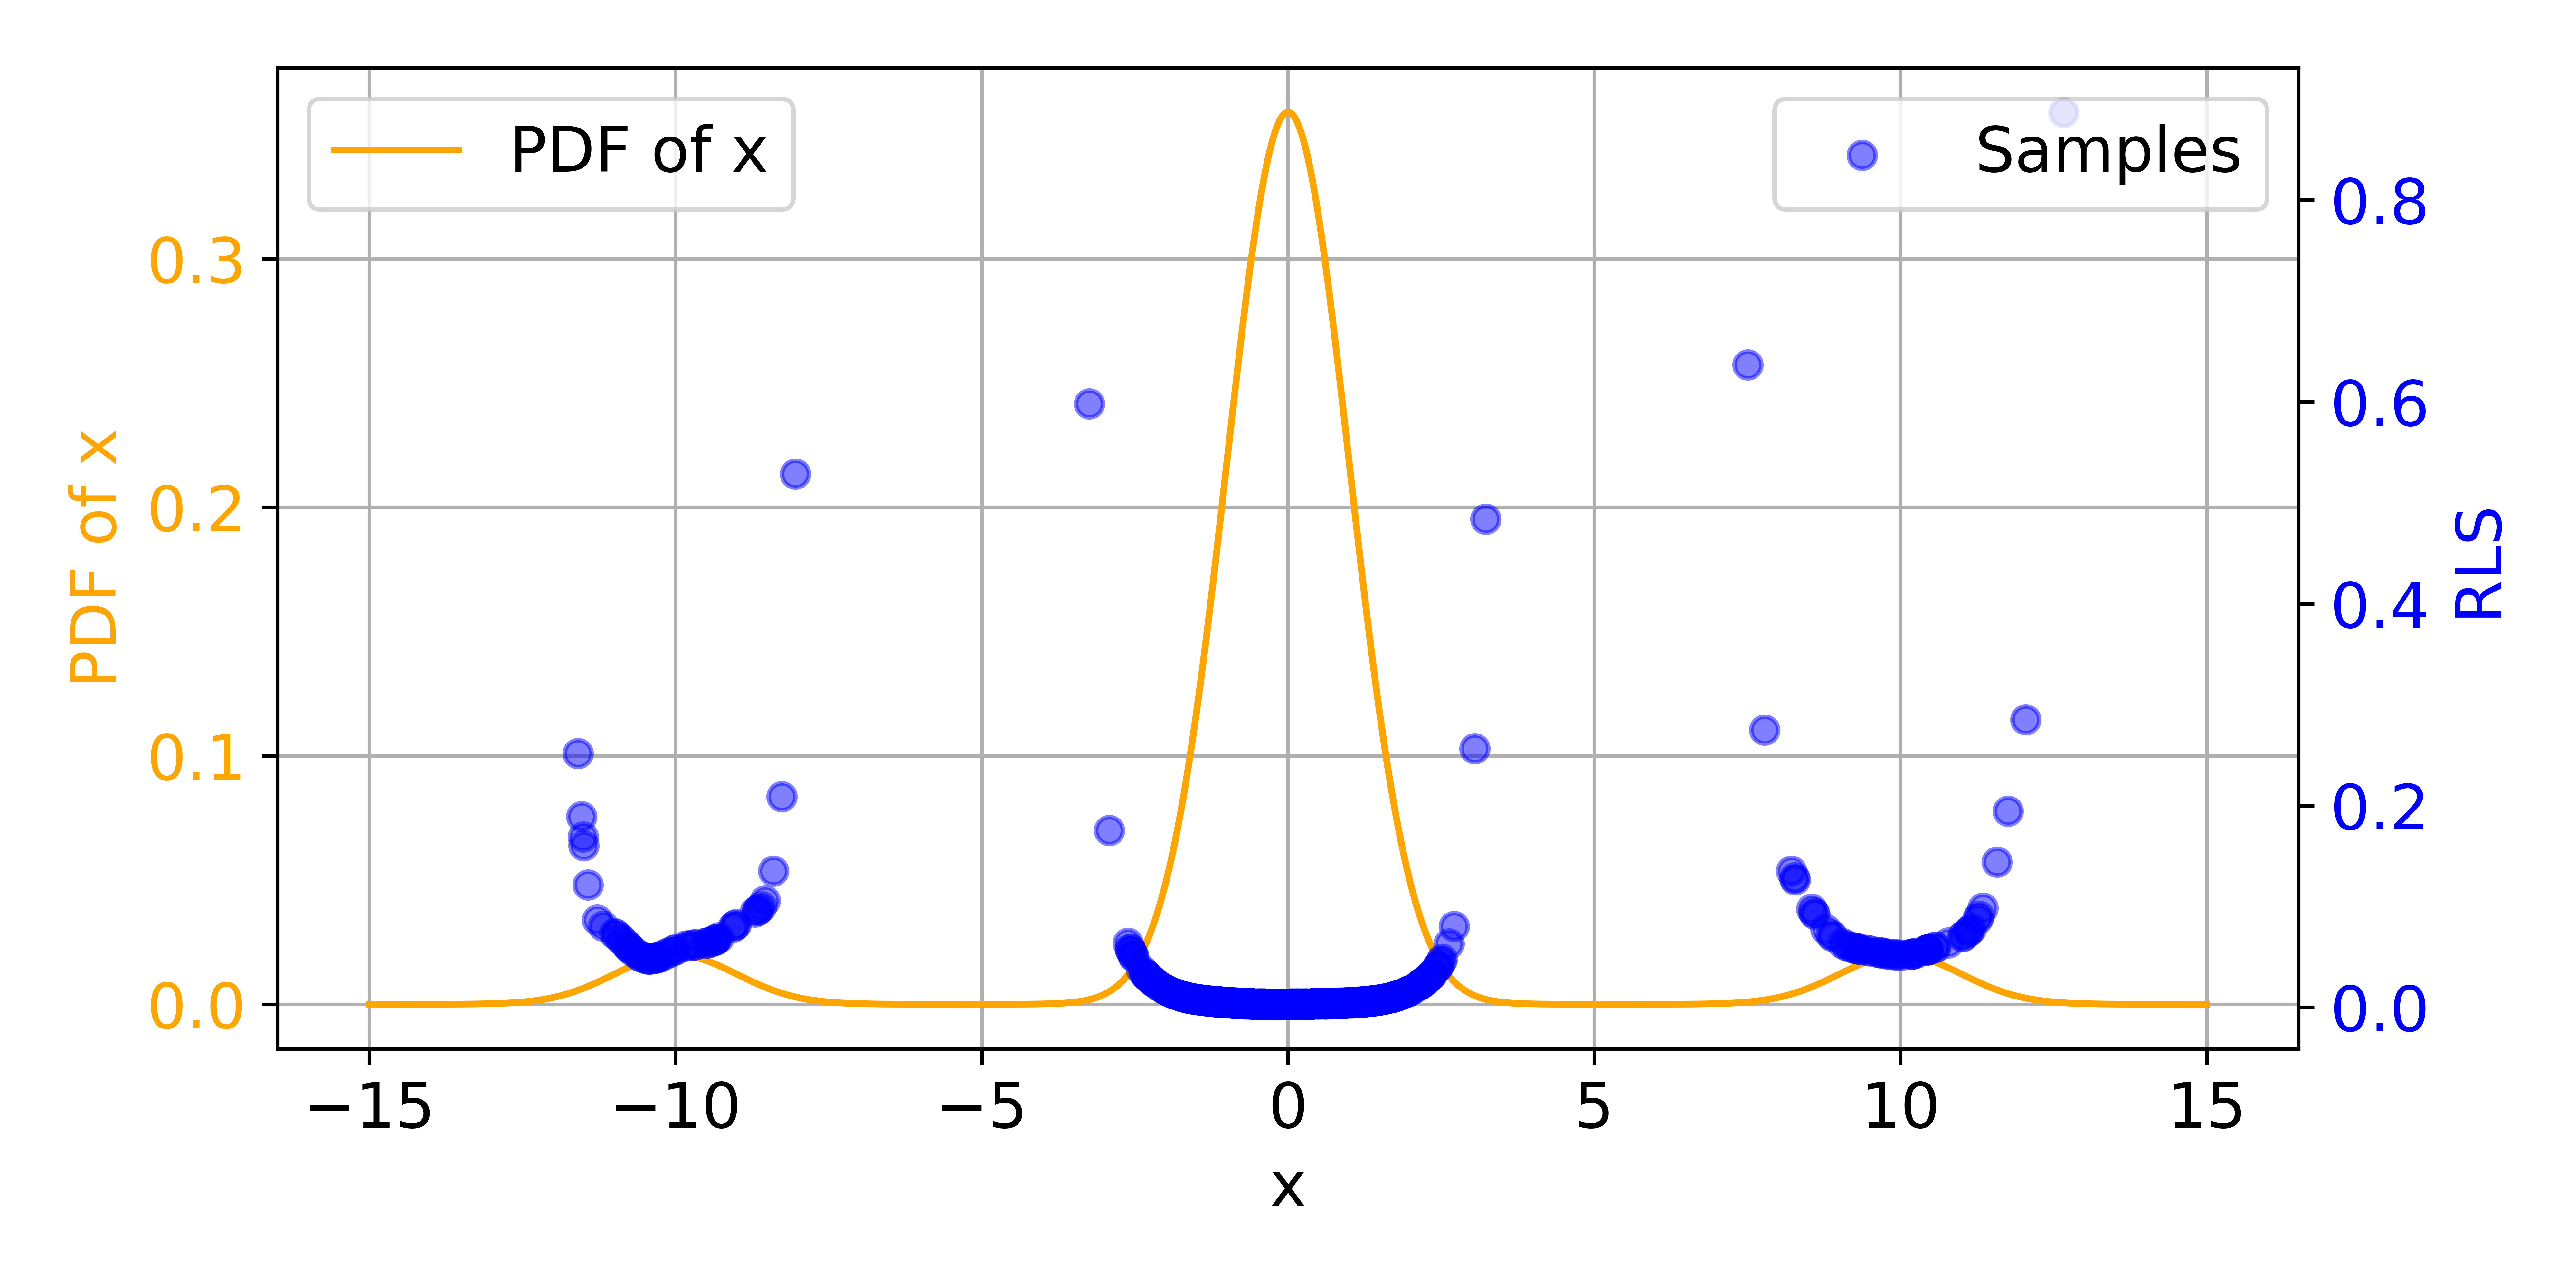
\includegraphics[width=0.8\linewidth]{Figures/Methods/rls-demo.png}
    \caption{A toy example illustrates using RLS sampling can help capture minority modes in the data. The orange curve depicts the PDF of a Gaussian mixture distribution with 1 majority mode in the middle and 2 minority modes on two sides, where the PDF is defined as $p=0.05\caN(-10,1) + 0.9\caN(0,1) + 0.05\caN(10,1)$. Blue points are a collection of random samples from that pdf, where the height of each point corresponds to the RLS for that individual point. RLSs are computed based on a Gaussian kernel with $\gamma=10^{-3}$ and $\sigma=3$. One can observe that samples from minority modes generally have higher RLSs, thus sampling based on the RLSs could contribute to balance the data. This figure is reproduced from \cite{schreursLeverageScoreSampling2022}.}
    \label{rls-demo}
\end{figure}

\subsection{Incorporating RLS sampling within the framework of Gen-RKM}
\label{subsec-methods-incor-rls-with-Genrkm}
The detailed sampling procedure based on RLSs in Gen-RKM is illustrated in this subsection. The main methodology is primarily developed based on \cite{schreursLeverageScoreSampling2022}, with some modifications applied due to differences in the model setting. We start by discussing two possible options for feature maps of RLS sampling in the framework of Gen-RKM.

\noindent\textbf{Feature map choices }\ To compute RLSs, a feature map function needs to be defined beforehand. Considering our work mostly focuses on learning image data, a more sophisticated similarity metric, typically a deep neural network, is preferred. Here we consider two different approaches for constructing feature maps.
\begin{itemize}
    \item \textbf{Shared explicit feature map with Gen-RKM: } Both Gen-RKM and RLS sampling are kernel based methods, meaning that they each have a feature map function projecting training data into feature space. Therefore the most natural way is to use the encoder part of Gen-RKM directly as feature map in RLS sampling. In this case, computation on RLS and Gen-RKM will share one same explicit feature map network: $\bvarphi(.)=\bphi(.)$ (recall that we denote feature map for Gen-RKM as $\bphi(.)$). This approach is preferred when no prior information is available.
    \item  \textbf{Explicit feature map based on a pre-trained classifier: } Another possible option is to use the next-to-last layer of a pre-trained classifier, such as ResNet18\cite{heDeepResidualLearning2016}, as the feature extractor. Similar ideas are proposed in \cite{schreursLeverageScoreSampling2022, zhangDeterminantalPointProcesses2017a}, where weighted sampling schemes are conducted based on the embeddings extracted from a pre-trained classifier. Some popular deep neural network models pre-trained on ImageNet\cite{dengImageNetLargescaleHierarchical2009} are readily implemented in \texttt{PyTorch} and \texttt{TensorFlow}. Notice that there is no need to fine-tune the pre-trained model on the exact training dataset, only forward pass operation is required to get image embeddings.
\end{itemize}

\noindent\textbf{Techniques for dimension reduction }\ Modern deep neural networks are characterized by their high dimensionality. For example, the output dimension of the next-to-last layer in AlexNet\cite{krizhevskyImageNetClassificationDeep2012} is 4096. Computation on RLSs can be rather demanding when the dimension of feature space is large. To improve computational efficiency, we introduce two dimension reduction techniques for different feature choices, as suggested in \cite{schreursLeverageScoreSampling2022}.
\begin{itemize}
    \item \textbf{Gaussian sketching: }\ Gaussian sketching is a ubiquitous approach in low-rank approximating large matrices in the field of randomized linear algebra. Let $\bZ$ be a Gaussian random matrix of size $d\times k$ where $k << d$, and $\bvarphi(\bX_{b})$ be a mini-batch of data with size $m$ after feature map in RLS sampling. The sketched matrix is simply given by multiplying the random matrix: 
    \begin{equation}
        \widetilde{\bvarphi}(\bX_{b}) = \bZ^{\top}\bvarphi(\bX_{b})\in \bbR^{m\times k}.
    \end{equation}
    This random projection guarantees that pairwise distances in the dataset are preserved in a much lower embedding space according to Johnson-Lindenstrauss lemma \cite{schreursLeverageScoreSampling2022}. One can refer to \cite{woodruffSketchingToolNumerical2014} for more technical details about sketching methods.
    \item \textbf{UMAP: }\ Uniform Manifold Approximation and Projection (UMAP) is a widely used non-linear dimensionality reduction technique developed by McInnes et al. \cite{mcinnesUMAPUniformManifold2020}. Compared to Gaussian sketching, UMAP can preserve more complex patterns in the data, though its training process is significantly slower.
\end{itemize}

\noindent\textbf{Modified training schemes based on RLS sampling }\ Detailed training algorithms based on RLS sampling are outlined in this subsection. For explicit feature map based on a pre-trained classifier, UMAP is preferred for dimension reduction in this case since RLSs are only computed once before the main training loop. The algorithm essentially follows the same principle as the inverse frequency sampling discussed earlier, i.e. performing weighted sampling under each mini-batch as well as resampling the full dataset for the final computation step, as presented in algorithm \ref{alg-rls-rkm-fixed}. 
\begin{algorithm}[H]
\caption{RLS Sampling in Gen-RKM with explicit feature map based on a pre-trained classifier}
\label{alg-rls-rkm-fixed}
\begin{algorithmic}[1]
\Require training data $\bD = \{\bx_i\}_{i=1}^{N}$; mini-batch size $m$; \\
regularization parameters $\eta, c_{\text{stab}}, \gamma_{RKM}$ for Gen-RKM; \\
explicit feature map $\bphi_{\btheta}(.)$ and explicit pre-image map $\bpsi_{\boldsymbol{\zeta}}(.)$ for Gen-RKM; \\
pre-trained classifier feature map $\bvarphi(.)$ and regularization $\gamma_{RLS}$ for RLS sampling; \\
dimension reduction size $k$
\LComment{Pre-compute RLS}
\State $\{\widetilde{\bvarphi}(\boldsymbol{x}_i)\}_{i=1}^{N} \gets \text{UMAP}_{k}(\{\bvarphi(\boldsymbol{x}_i)\}_{i=1}^{N})$ \Comment{get UMAP embeddings}
\State $l_i \gets \widetilde{\bvarphi}(\boldsymbol{x}_i)^\top(\bS_{\Tilde{\bvarphi}}+\gamma_{RLS}\mathbf{I})^{-1}\widetilde{\bvarphi}(\boldsymbol{x}_i)$ \Comment{Compute leverage scores}
\State $p_i \gets l_i / \sum_{j=1}^n l_j$
\LComment{Training loop}
    \For {each epoch}
        \For{each mini-batch $B \subset \bD$}
        \State $B \gets$ sample a mini-batch of size $m$ with probability $\boldsymbol{x}_i \sim p_i$ 
        \State do step 6-11 in algorithm \ref{alg-gen-rkm-dual}
        \EndFor
    \EndFor
\LComment{Modified final computation step in Gen-RKM}
\State $\bD_{\text{resampled}} \gets$ resample the full dataset with probability $\bx_i \sim p_i$ 
\State repeat step 7-9 in algorithm \ref{alg-gen-rkm-dual}  on $\bD_{\text{resampled}}$
\end{algorithmic}
\end{algorithm}

For the RLS sampling using a shared feature map with Gen-RKM, RLSs are recomputed in each iteration since the feature map for RLS is not fixed (i.e. parameters of feature map network need to be updated with every iteration). To alleviate the computational load, Gaussian sketching is implemented to reduce the dimension of the feature map. Sketching is considerably fast even when performed in every iteration, due to the simplicity of matrix multiplication involved. In addition, a two-stage sampling procedure is applied as suggested in \cite{schreursLeverageScoreSampling2022}. First, a subset of training data is uniformly sampled (we set the size of this subset to be 20 times the mini-batch size), and RLSs are computed only for that core set. In the second stage, a mini-batch is sampled based on the calculated RLSs of this core set for training. The detailed implementation is shown in algorithm \ref{alg-rls-rkm-shared}. Likewise in the previous setting, the final computation step in Gen-RKM is conducted based on the RLS-resampled dataset.
\begin{algorithm}[H]
\caption{RLS Sampling in Gen-RKM with a shared feature map}
\label{alg-rls-rkm-shared}
\begin{algorithmic}[1]
\Require training data $\bD = \{\bx_i\}_{i=1}^{N}$; mini-batch size $m$; \\
regularization parameters $\eta, c_{\text{stab}}, \gamma_{RKM}$ for Gen-RKM; \\
explicit feature map $\bphi_{\btheta}(.)$ and explicit pre-image map $\bpsi_{\boldsymbol{\zeta}}(.)$ for Gen-RKM; \\
regularization parameter $\gamma_{RLS}$ for RLS sampling and dimension reduction size $k$;
\LComment{Training loop}
    \For {each epoch}
        \For{each mini-batch $B \subset \bD$}
        \LComment{two-stage sampling procedure}
        \State $\bD_{s} \gets$ uniformly sample a subset from $\bD$ with size $20*m$ 
        \State $\widetilde{\bphi}_{\btheta}(\bx_i) \gets \bZ_k^\top\bphi_{\btheta}(\bx_i),\quad \text{s.t.}\bx_i\in \bD_s$ \Comment{Gaussian sketching}
        %\LComment{Compute RLS on $\bD_{s}$ under each iteration}
        \State $l_i \gets \widetilde{\bphi}_{\btheta}(\bx_i)^\top(\bS_{\widetilde{\bphi}_{\btheta}}+\gamma_{RLS}\mathbf{I})^{-1}\widetilde{\bphi}_{\btheta}(\bx_i)$
        \State $p_i \gets l_i / \sum_{j=1}^{20m} l_j$
        \State $B \gets$ sample a mini-batch of size $m$ with probability $\bx_i \sim p_i$
        \State do step 6-11 in algorithm \ref{alg-gen-rkm-dual}
        \EndFor
    \EndFor
\LComment{Compute final RLS on full dataset}
\State $\widetilde{\bphi}_{\btheta}(\bx_i) \gets \bZ_k^\top\bphi_{\btheta}(\bx_i),\quad \text{s.t.}\bx_i\in \bD$
\State $l_i^{\text{final}} \gets \widetilde{\bphi}_{\btheta}(\bx_i)^\top(\bS_{\widetilde{\bphi}_{\btheta}}+\gamma_{RLS}\mathbf{I})^{-1}\widetilde{\bphi}_{\btheta}(\bx_i)$
\State $p_i^{\text{final}} \gets l_i^{\text{final}} / \sum_{j=1}^N l_j^{\text{final}}$
\LComment{Modified final computation step in Gen-RKM}
\State $\bD_{\text{resampled}} \gets$ resample a dataset of size $N$ with probability $\bx_i \sim p_i^{\text{final}}$ 
\State repeat step 7-9 in algorithm \ref{alg-gen-rkm-dual}  on $\bD_{\text{resampled}}$
\end{algorithmic}
\end{algorithm}

\subsection{Extension: Other measurement for imbalance sampling}
\label{subsec-methods-islation-forest}
As mentioned in Section \ref{subsec-lr-unbalance-super-unsuper}, many studies focus on anomaly detection in unsupervised learning settings. These experiences can be leveraged to address the issue of imbalanced data within the Gen-RKM framework. In addition to the ridge leverage score, which assesses the importance of individual observations in a dataset, other anomaly detection methods can be utilized to measure the uniqueness or anomaly level of observations. Subsequently, re-sampling can be carried out based on the uniqueness of each sample, similar to the approach used in ridge leverage score sampling. 

Isolation forest (Iforest)\cite{liu2008isolation}, as mentioned in Section \ref{subsec-lr-unbalance-super-unsuper}, provides an assessment for the degree of the anomaly of each data point as follows,
\begin{align}
&S(x, n) = 2^{-\frac{h(x)}{c(n)}}\label{ascore} \\
&c(n) = 2H(n-1) - \frac{2(n-1)}{n} \\
&H(k) = \ln(k) + \xi
\end{align}
where \begin{itemize}
    \item $S(x, n)$ represents the anomaly score of data point $x$, $n$ is the number of samples. The larger the score, the higher the likelihood that $x$ is considered an anomaly or outlier. 
    \item $h(x)$ is the path length required to isolate point $x$ in the isolation forest. Shorter path lengths suggest that $x$ is easier to isolate, thus potentially being an outlier.
    \item $c(n)$ is the average path length under normal conditions for a sample size $n$. This calculation takes into account the balance and imbalance factors of a binary search tree.
    \item $H(k)$  is a harmonic number, typically used to estimate the average path length of binary search trees. And $\xi$ is the Euler-Mascheroni constant, approximately 0.5772156649.
\end{itemize}
We can easily integrate isolation forest anomaly score sampling (Iforest sampling) into the Gen-RKM framework to address the imbalance data problem by simply replacing steps 3-4 in Algorithm \ref{alg-rls-rkm-fixed} with the computation of anomaly scores using an isolation forest model (see $S(x, n)$ in equation \ref{ascore}) based on the extracted features from the feature map,  while maintaining all other steps unchanged. Note that this is only applicable with a pre-trained classifier-based feature map, as it allows the isolation forest to be fitted just once in the algorithm.



